\documentclass{beamer}
\usepackage{tikz}
\usetikzlibrary{shapes}
\usetheme{Madrid}

\tikzstyle{startstop} = [ellipse,draw]
\tikzstyle{normal} = [rectangle,draw,text centered]
\tikzstyle{decision} = [diamond,aspect=4,draw]
\tikzstyle{io} = [trapezium, trapezium left angle=70, trapezium right angle=110,draw]

\title[beamer class]{Practice on Beamer and Tikz}
\author[arko]{Preetom Saha Arko}
\institute[BUET]{Bangladesh University of Engineering and Technology}
\date{\today}

\begin{document}
	\frame{\titlepage}
	\begin{frame}
		\frametitle{Introduction to Beamer}
		\begin{itemize}
			\item Beamer is very important for technical presentation. \pause
			\item Beamer provides fixed typesetting.
		\end{itemize}
	\end{frame}
	
	\begin{frame}
		\frametitle{Columns}
		\begin{columns}
			\column{0.5\textwidth}
			Tikz is an important tool for creating self-generated figures.
			$ E=mc^2 $
			\column{0.5\textwidth}
			Today we will cover both beamer and tikz.
		\end{columns}
	\end{frame}
	
	\begin{frame}
		\begin{alertblock}{Block Header}
			Here are some text inside block.
		\end{alertblock}
	\end{frame}
	
	\begin{frame}
	\begin{figure}[h]
		\centering
		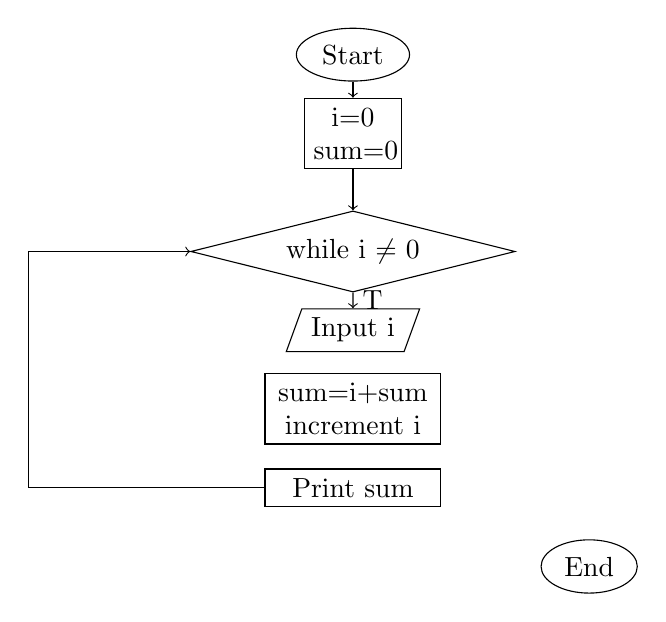
\begin{tikzpicture}
		%\draw (0,1) -- (5,4);
		%\draw (0,1) -| (5,4);
		%\draw (0,1) -- (5,1) -- (5,4) -- cycle;
		%\draw (6,2) rectangle (9,4);
		%\draw (0,0) circle[radius=3];
		%\draw (0,0) ellipse[x radius=3,y radius=2];
		%\draw (2,3) -- ++(3,2);
		\node[startstop](start) {Start};
		\node[normal,below of=start, text width=1cm](i_sum) {i=0  sum=0};
		\node[decision,below of=i_sum,yshift=-0.5cm](while) {while i $ \neq $ 0};
		\node[io,below of=while](input) {Input i};
		\node[normal,below of=input,text width=2cm](sum_incr) {sum=i+sum increment i};
		\node[normal,below of=sum_incr,text width=2cm](print) {Print sum};
		\node[startstop,below of=print,right of=print,xshift=2cm](end) {End};
		
		\draw[->] (start) -- (i_sum);
		\draw[->] (i_sum) -- (while);
		\draw[->] (while) -- node[right] {T} (input);
		\draw[->] (print.west) -- ++(-3,0) |- (while.west);
		\end{tikzpicture}
	\end{figure}
	
	\end{frame}
	
\end{document}